\section{Bivariate Correspondence Analysis}
\label{sec:bivariate}

Chess game can end in three different ways. Player can win, lose or game can be a draw. In this section I study using attraction repulsion matrix and bivariate correspondence analysis how color of chess pieces, chess variant and time of the day affect the game result. I have selected only those standard and crazyhouse chess games in which my opponent have been at least 100 rating points stronger than me.

In figure \ref{fig:color vs result} a heat map presentation of an attraction repulsion matrix between color of chess pieces and game result is shown. I can see that when playing with white pieces I win more often than when playing with black pieces. I also see that interestingly having black pieces makes slightly more probable for the game to end in a draw.

\begin{figure}[ht!]
    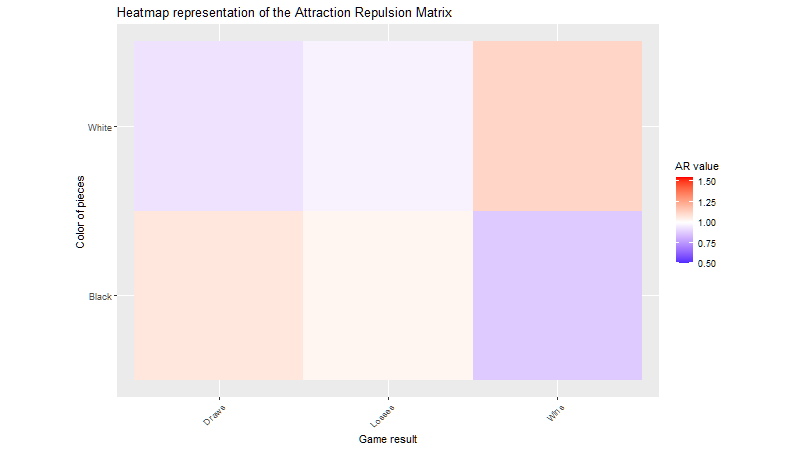
\includegraphics[width=\textwidth]{../img/color_and_result.png}
    \caption{Heat map presentation of attraction repulsion matrix between color of chess pieces and game result.}
    \label{fig:color vs result}
\end{figure}

In figure \ref{fig:variant vs result} a visualization of correspondence analysis between chess variant and game result is shown. I see that game ending in a draw is mostly related to classical chess as crazyhouse variant vector points strictly to opposite direction from draw vector. It must be noted that there are much fewer games ending in a draw than games ending in win or loss which makes draw arrow very long in the visual representation. Figure also suggest a weak connection that losing and playing crazyhouse chess are related to each other and winning is related to Standard chess. This is consistent with winning probabilities given in table \ref{tbl:results by variant} but a bit surprising when comparing to figure \ref{fig:winning probabilities} which would suggest that there still exist lot of "probability mass" for winning against strong opponents in crazyhouse chess.

\begin{figure}[ht!]
    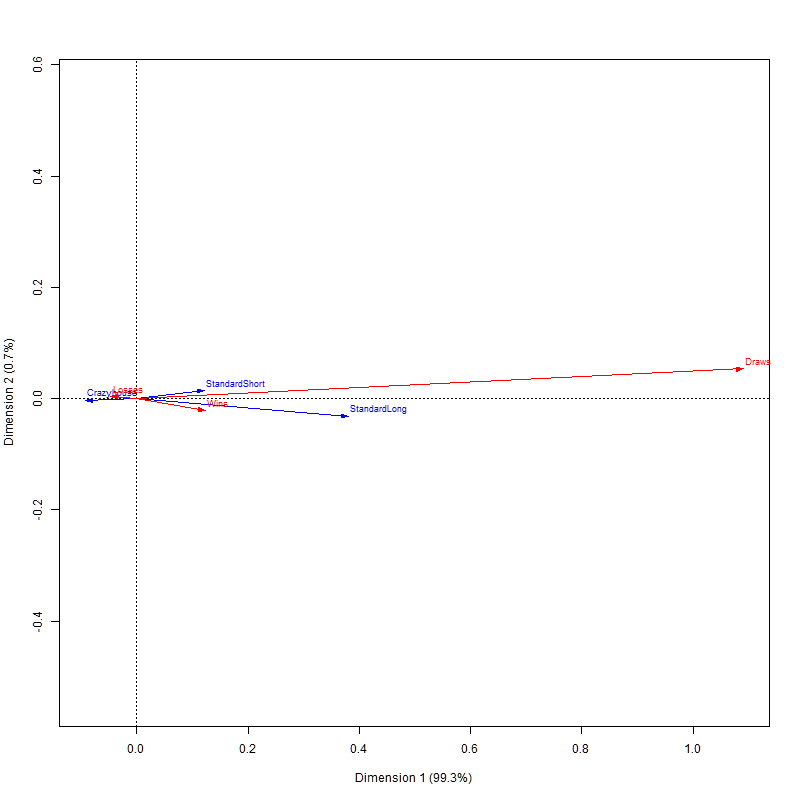
\includegraphics[width=\textwidth]{../img/variant_and_result.png}
    \caption{Visualization of correspondence analysis between chess variant and game result.}
    \label{fig:variant vs result}
\end{figure}

In figure \ref{fig:time vs result} a visualization of correspondence analysis between time of the day and game result is shown. Game has been given label "morning" if it is played before 12 o'clock, label "day" if it is played after 12 o'clock and before 18 o'clock and label "evening" if it has been played after 18 o'clock. This figure shows that in general time of the day and game result doesn't have strong connection despite the small spike in performance at afternoon seen in figure \ref{fig:games vs time of day}. This effect is lost in data aggregation to three categories. Draws and mornings are aligned in the image. I think this is caused by my preference to play longer standard games in morning as standard games tend to end more often in draws than for example in crazyhouse games.

\begin{figure}[ht!]
    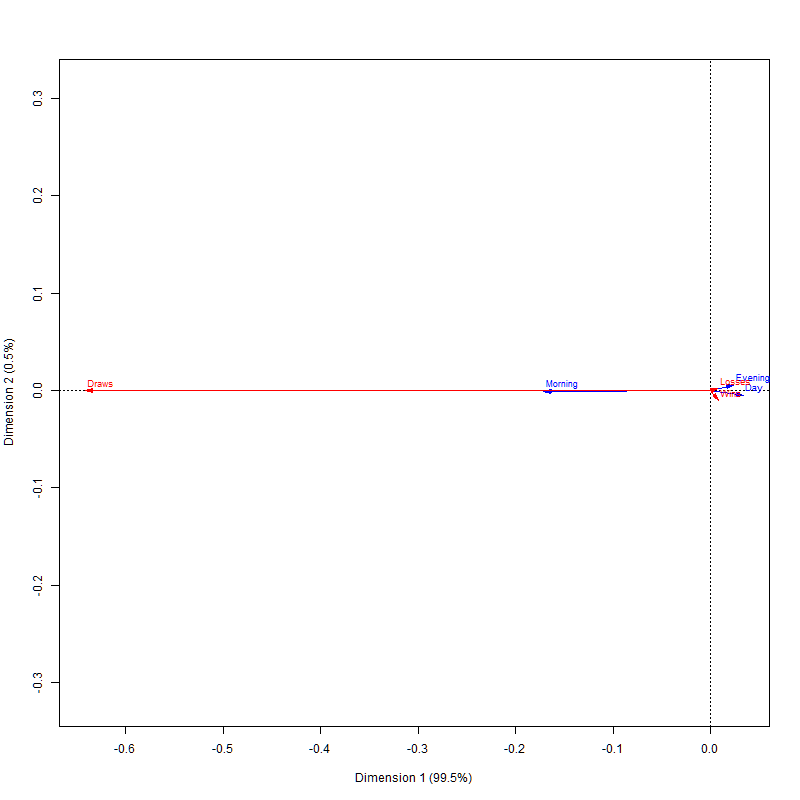
\includegraphics[width=\textwidth]{../img/time_and_result.png}
    \caption{Visualization of correspondence analysis between time of the day and game result.}
    \label{fig:time vs result}
\end{figure}